\chapter{Titolo del terzo capitolo}
\label{chap:cap3}
%Quando parliamo di \emph{modellizzazione ad agenti} intendiamo un tipo di modellizzazione computazionale nel quale un fenomeno viene rappresentato in termine di quelli che vengono chiamati agenti e delle loro interazioni; con \emph{agente} andiamo ad indicare un individuo o un oggetto autonomo in possesso di determinate proprietà e in grado di compiere certe azioni. \\I rapporti fra le varie entità che popolano il modello avvengono localmente, cioè solo fra quelli che vengono considerati \emph{vicini}: è immediato, pertanto, pensare che i soggetti sotto esame si muovano su di una rete e che possano necessariamente avere a che fare solo con chi si trova in loro prossimità. \\ Il primo grande vantaggio derivante dall'uso di questo approccio risiede nel fatto che risulta di più semplice comprensione rispetto ad una rappresentazione di tipo matematico: dal momento che consente di proiettare negli agenti quella che è la nostra esperienza personale, modulata in termini delle interazioni con gli individui coi quali entriamo in contatto, è evidente quanto possa essere più vicino al nostro linguaggio e al nostro modo di pensare. D'altro conto, non si può negare che un'equazione, se risolubile, fornisce in modo diretto un risultato senza il bisogno di far girare un modello, che, specialmente se costituito di un gran numero di agenti, può richiedere un tempo di esecuzione talmente lungo da renderlo poco funzionale \cite{Rand}. Un ulteriore merito del quale è necessario prendere atto è la sua capacità di mettere in luce il fenomeno dell'\emph{emergenza}, cioè di tutto quell'insieme di comportamenti e proprietà che vengono fuori dall'interazione di singoli individui e che non risultano predicibili a partire dalle caratteristiche di questi ultimi; ciò è possibile perché si tratta di un approccio "across-levels", secondo il quale gli agenti non vengono considerati avulsi dall'ambiente in cui sono immersi, ma viene dato particolare rilievo alla reciproca influenza fra i due. \\ Non sarà sorprendente, a questo punto, affermare che il processo di modellizzazione sottostà ad una serie di passi che possono venire iterati più volte - dando luogo a quello che chiamiamo "modeling cycle" - in modo da rendere il modello il più efficace ed efficiente possibile:
%\begin{enumerate}
%\item \textit{formulazione delle domande}, per meglio mettere a fuoco il problema che si vuole analizzare;
%\item \textit{costruzione delle ipotesi}, che devono inizialmente essere il più semplici possibili, per venir poi rinforzate ed arricchite più avanti nel processo;
%\item \textit{scelta delle variabili di stato e dei parametri}, per iniziare a mettere per iscritto il modo in cui ci aspettiamo che il nostro modello si comporti;
%\item \textit{implementazione del modello}, che consente di esplorare e valutare se le assunzioni fatte sono valide ed hanno prodotto un che di utile;
%\item \textit{analisi, test e revisione}, così da apportare modifiche o migliorie;
%\item \textit{comunicazione del modello} \cite{Grimm}.
%\end{enumerate}
%In ultimo, è interessante sottolineare, seppur brevemente, quale sia il ruolo epistemico della simulazione computazionale: è, infatti, possibile attribuirle un potere sia \emph{esplicativo}, poiché permette di comprendere come si siano verificati alcuni eventi, sia \emph{predittivo}, dal momento che rende possibile immaginare il comportamento futuro di un sistema sotto determinate circostanze, che \emph{esplorativo}, in quanto fa sì che le informazioni che intendiamo rappresentare possano essere condivise e rese note ad altri \cite{Primiero}.
%\\ All'interno di questo lavoro di tesi faremo uso di Netlogo, che è sia un IDE, ovvero un ambiente di sviluppo integrato, che un linguaggio di modellazione; è stato progettato nel $ 1999 $ col fine di rendere il più semplice possibile la costruzione di modelli basati su agenti. Nella fattispecie, utilizzeremo la versione $ 6.2.0 $; per ulteriori dettagli tecnici, rimandiamo alla documentazione ufficiale \cite{Wilensky}.
Un elemento sul quale vorremo concentrare la nostra attenzione è la \emph{percezione del rischio}, poiché ci aspettiamo che possa rappresentare un fattore chiave nell'andamento dell'epidemia. Si osserva, infatti, che, qualora ci si trovi di fronte ad una malattia i cui sintomi sono evidentemente manifesti, le persone modificano il proprio comportamento e le proprie abitudini sulla base della propria soggettiva sensazione di pericolo; ad esempio, potrebbero prediligere l'uso di un mezzo di trasporto privato, rispetto ad uno pubblico, per recarsi a lavoro, in modo da limitare le occasioni di contatto con estranei. È altresì vero che la percezione del rischio varia anche col grado di intimità che si ha con un determinato individuo: in linea di massima, la tendenza è quella di temere meno l'infezione se ci si trova in compagnia di un familiare o di un amico, mentre in presenza di estranei il livello di allerta si fa ben più alto. \\Per amore di semplicità, in questo lavoro assumeremo che tutti i soggetti percepiscano il rischio e reagiscano ad esso allo stesso modo: facciamo, cioè, un'ipotesi di \emph{popolazione omogenea}. Aggiungiamo due ulteriori supposizioni:
\begin{enumerate}
	\item la malattia si rende visibile nel medesimo momento in cui infetta qualcuno;
	\item la percezione del rischio è proporzionale alla frazione di contatti con individui infetti rispetto alla totalità dei contatti \cite{Bagnoli2007}.
\end{enumerate}
Poniamo la nostra attenzione su reti costituite da $ N $ nodi e $ 2mN $ link. Come già fatto in precedenza, andiamo ad indicare con $ a_{ij} $ l'ij-esimo elemento della matrice di adiacenza - pari a 1 se esiste un arco da j a i e $ 0 $ altrimenti - e con $ k_i = \sum_{j} a_{ij} $ la connettività del sito $ i $ - così che risulta $ \langle k \rangle = 2m $ - ; denotiamo, invece, quella dei suoi vicini come $ j_{1}^i \dots j_{k_{i}}^i $. Andiamo a sostituire alla probabilità d'infezione netta, indicata con la lettera $ \tau $, la quantità $ u\left(s,k \right) $: nello specifico, questa può esplicitamente essere scritta come
\begin{equation}
	u\left(s,k_i \right) = \tau \exp(-J \tfrac{s}{k_i})
	\label{infect_sk}
\end{equation}
e va a rappresentare la probabilità che il sito $ i $, avente connettività $ k_i $, contragga l'infezione da uno degli $ s $ vicini malati \cite{Bagnoli2014}. Quanto appena scritto riflette in pieno quanto asserivamo poco sopra, ovvero che l'eventualità di venire contagiati diminuisca in funzione della percezione del rischio, data dalla percentuale di vicini infetti e modulata da un fattore $ J $, che può dipendere dal tipo di misure di precauzione adottate. 
%\section{Approssimazione di campo medio}
\\La più semplice approssimazione di campo medio che è possibile formulare richiede di trascurare l'eventuale correlazione fra le variabili; in altre parole, si assume che non ci siano loop. 
\\Poniamoci nel caso in cui la rete che rappresenta i contatti sia aleatoria e che $ k $ sia fissato: allora, se indichiamo con $ c $ la frazione di infetti al tempo $ t $ e con $ c' $ quella al tempo immediatamente successivo $ t + 1 $, possiamo scrivere che
\begin{equation}
c' = \sum_{s = 0}^k \binom{k}{s}c^s \left(1-c \right)^{k-s} p\left(s,k \right),
\end{equation}
laddove $ p\left(s,k \right) = 1 - \left[1 - u \left(s,k \right) \right]^s$ è la probabilità di ammalarsi se sono presenti $ s $ vicini infetti su $ k $ \cite{Bagnoli2014}. 
\medskip
\\Apriamo, a questo punto, una doverosa parentesi ed introduciamo un ulteriore concetto caro alla teoria dei grafi: la \emph{percolazione}, ovvero la rimozione di un vertice di una rete (p. \emph{di sito}) oppure quella di un arco (p. \emph{di legame}). In questo contesto, possiamo affermare che un link viene occupato con una probabilità $ \phi $; link di questo tipo sono quelli lungo cui può essere trasmessa l'infezione. Al crescere di  $ \phi $, nodi inizialmente isolati si fanno via via più grandi, fino ad arrivare a creare un cluster unico  che altro non è se non quella che abbiamo chiamato componente gigante e che raggiunge la sua dimensione massima per $ \phi = 1 $; questo fenomeno prende il nome di \emph{transizione di percolazione}. Quello che si può arrivare a dire è che la soglia di percolazione su di una rete coincide con la soglia epidemica per la diffusione di una malattia sulla medesima rete: infatti, per valori piccoli di $ \phi $ il primo infetto appartiene necessariamente ad un cluster di dimensioni modeste e, di conseguenza, la maggior parte della popolazione non viene infettata; al contrario, quando $ \phi $ è grande, aumenta il numero di vertici facenti parte della componente gigante e, di pari passo, la probabilità che il paziente zero vi faccia parte e dia l'avvio ad una vera e propria ondata epidemica \cite{Newman}.
\medskip
\\Torniamo al nostro problema. Ci aspettiamo che in prossimità della soglia di percolazione/epidemica la \eqref{infect_sk} sia piccola, il che ci consente di approssimare
\begin{equation}
	c' \simeq \sum_{s = 0}^k \binom{k}{s}c^s \left(1-c \right)^{k-s} s \tau exp(-J \tfrac{s}{k});
\end{equation}
ponendo $ a \doteq exp(- \tfrac{J}{k}) $, si può finire per trovare che
\begin{equation}
	c' = \tau a k \left(c a + 1 - c \right)^{k-1}.
\end{equation}
La soglia critica $ J_c $ corrisponde allo stato stazionario $ c = c' $, nel limite $ c \rightarrow 0 $:
\begin{equation}
	\tau = \frac{1}{k} exp(\tfrac{J_c}{k}),\quad J_c = k \ln(k \tau).
\end{equation}

\begin{figure}[t]
		\begin{center}
			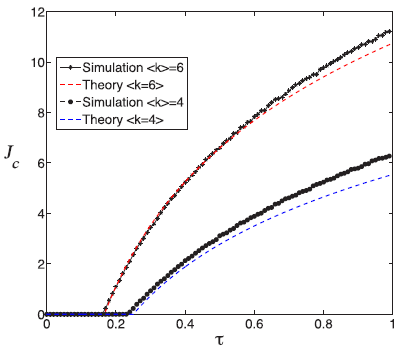
\includegraphics[scale=.8, keepaspectratio]{mean_field_sim}
			\caption{Confronto fra l'approssimazione di campo medio e le simulazioni condotte per una rete aleatoria al variare di $ \langle k \rangle $ \cite{Bagnoli2014} .}
			\label{fig:sim}
		\end{center}
\end{figure}
La nostra predizione è piuttosto precisa: ce lo confermano le simulazioni eseguite, come possiamo osservare in \cref{fig:sim}.